\documentclass[12pt,a4paper]{article}
\usepackage[utf8]{inputenc} % sempre salve seus arquivos como UTF8
\usepackage[T1]{fontenc}
\usepackage[english]{babel}

\usepackage[left=2.5cm,right=2cm,top=2cm,bottom=2.5cm]{geometry}
\usepackage{amsmath}
\usepackage{amsthm}
\usepackage{amsfonts}

\usepackage{graphicx}
\usepackage{algorithm}
\usepackage{color}
\usepackage[noend]{algpseudocode}
\usepackage{mathtools}
\usepackage{subfig}
\usepackage{diagbox}

% load times font
\usepackage{mathptmx}
\usepackage[scaled=.90]{helvet}
\usepackage{courier}

% comandos
\newcommand{\mdc}[1]{\mathrm{mdc}(#1)}

\DeclarePairedDelimiter\ceil{\lceil}{\rceil}
\DeclarePairedDelimiter\floor{\lfloor}{\rfloor}

% Foot without marker
\newcommand\blfootnote[1]{%
	\begingroup
	\renewcommand\thefootnote{}\footnote{#1}%
	\addtocounter{footnote}{-1}%
	\endgroup
}

\title{MO446 -- Introduction to Computer Vision  \\ Project 4}
\author{Breno Leite  \\ Guilherme Leite}
\date{26/10/2017}

\begin{document}

\maketitle
\blfootnote{\textit{\textbf{Important note:} The borders seen in the figures are not part of the image, they are figurative information about the starting and ending points of the image. Moreover, all the image scales in this report were changed in order to make the text more readable.}} \\

%% ---------------- Starts here --------------------------------

\textbf{\LARGE Question 3 - Image Descriptor}\\

	In this question we extracted the descriptor of all the images in the data set and saved these descriptors in a file, so the next time the program was executed it could load the descriptors, and perform faster, instead of recalculating every descriptor again.

	An image descriptor consist of all the regions in an image and their information. To extract all these regions, firstly we used OpenCV's implementation of the Kmeans algorithm, check Figure \ref{fig:kmeans}.

\newpage

\begin{figure}[!h]
	\centering
	\subfloat[K = 2.]{
		{
			\setlength{\fboxsep}{1pt}
			\setlength{\fboxrule}{1pt}
			\fbox{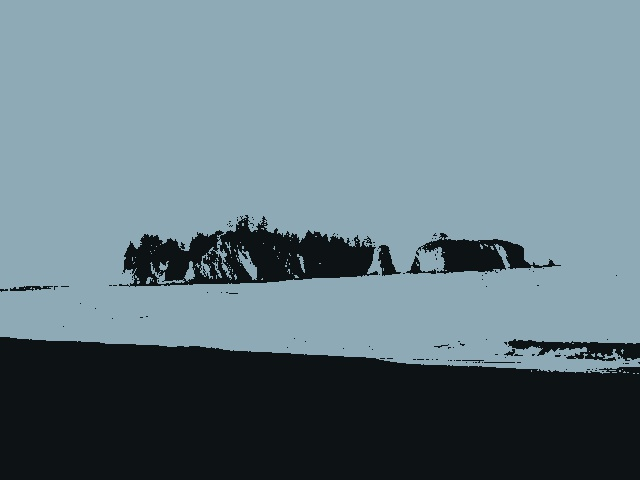
\includegraphics[scale=0.3]{report/p4-3-0-K02}}
		}
		\label{fig:kmeans02}
	}
	\quad
	\subfloat[K = 5.]{
		{
			\setlength{\fboxsep}{1pt}
			\setlength{\fboxrule}{1pt}
			\fbox{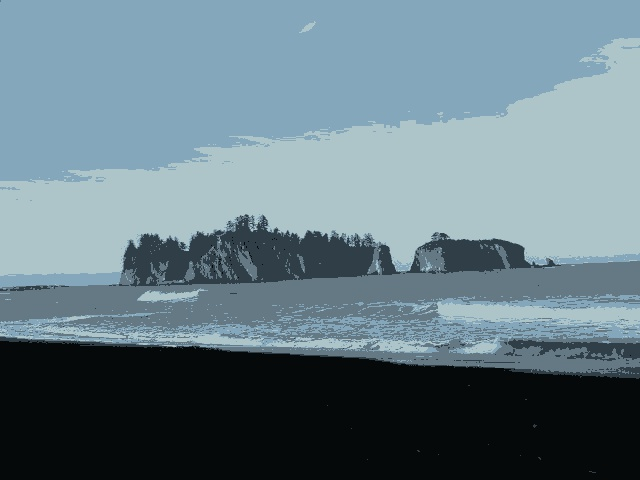
\includegraphics[scale=0.3]{report/p4-3-0-K05}}
		}
		\label{fig:kmeans05}
	}
	\quad
	\subfloat[K = 8.]{
		{
			\setlength{\fboxsep}{1pt}
			\setlength{\fboxrule}{1pt}
			\fbox{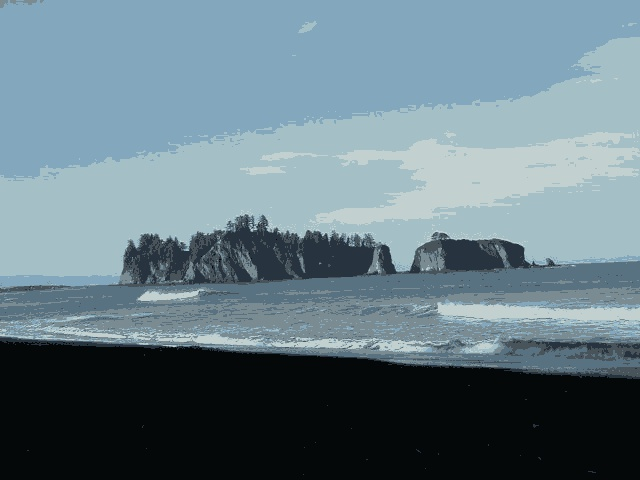
\includegraphics[scale=0.3]{report/p4-3-0-K08}}
		}
		\label{fig:kmeans08}
	}
	\quad
	\subfloat[K = 10.]{
		{
			\setlength{\fboxsep}{1pt}
			\setlength{\fboxrule}{1pt}
			\fbox{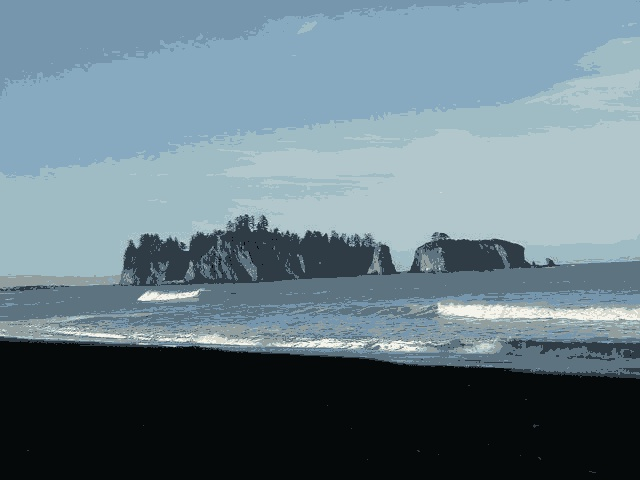
\includegraphics[scale=0.3]{report/p4-3-0-K10}}
		}
		\label{fig:kmeans10}
	}
	\caption{Regions extracted with Kmeans implemented by OpenCV, using different $K$ values.}
	\label{fig:kmeans}
\end{figure}

	The algorithm returns K regions extracted based only in their colours and intensity, in Figure \ref{fig:kmeans} each colour represents a region. The number of regions ($K$) was selected by trial and error, a small $K$ yields big generic regions, as in Figure \ref{fig:kmeans02} for example the sky and the ocean were blended into a single region, which is not helpful to discriminate this image, in contrast a big $K$ yields many small regions as seen in Figure \ref{fig:kmeans10},  too small regions don't really increase the matching accuracy, the reason will be explained later on, although they increase the computation time significantly. The best results for the images analysed were yielded by a value of $K = 5$ regions, seen in Figure \ref{fig:kmeans05}.

	One example of why $K = 5$ is better is the comparison between the sky in Figure \ref{fig:kmeans05} and Figure \ref{fig:kmeans08}, in the former it is possible to distinguish around two colours for the sky region, a light and a dark blue, as in the later the sky was sub-divided into roughly three regions, but a pixel by pixel analysis reveals more regions describing the sky and that won't really improve the matching process.

	The ideal $K$ value can vary from image to image, and there is a method to minimise between the tested values using silhouette analysis. As in this project the $K$ value was set based on empirical evidence extracted from the data set distributed with the project description.

	In order to use these regions as an image descriptor, it is desired that each region is descriptive enough to highlight a feature. The regions returned by Kmeans are still too generic, some of them are even disconnected into clusters in opposite corners of the image, as in Figure \ref{fig:kmeans05} the sky and some waves possess the same colours and so are seen as the same region, even though they are disconnected and represent different things in the image.

\newpage

	To eliminate these disconnected regions we ran a BFS explorer in the entire image. The BFS returns every connected region separately, which receives a new label, eliminating disconnected regions altogether, Figure \ref{fig:bfs} shows the returned regions.
	The borders remained unchanged during this process, but reducing their noise could improve the expression of some regions, increasing the accuracy of the solution.

\begin{figure}[!h]
	\centering
	\subfloat[X = 0.]{
		{
			\setlength{\fboxsep}{1pt}
			\setlength{\fboxrule}{1pt}
			\fbox{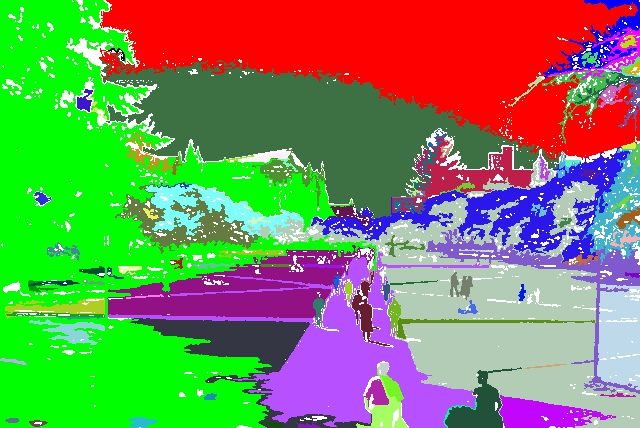
\includegraphics[scale=0.3]{report/p4-3-1-X00}}
		}
		\label{fig:bfs00}
	}
	\quad
	\subfloat[X = 6.]{
		{
			\setlength{\fboxsep}{1pt}
			\setlength{\fboxrule}{1pt}
			\fbox{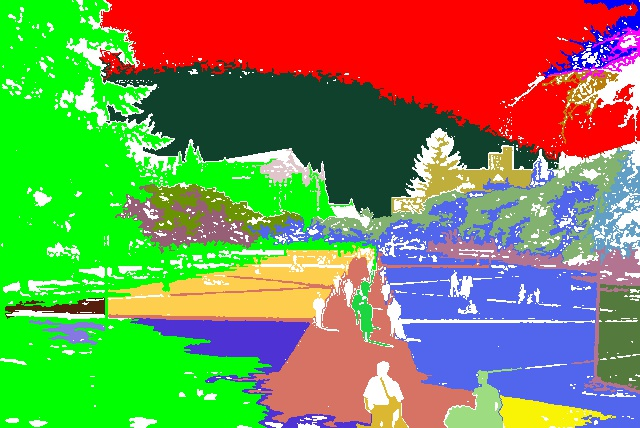
\includegraphics[scale=0.3]{report/p4-3-1-X06}}
		}
		\label{fig:bfs06}
	}
	\quad
	\subfloat[X = 10.]{
		{
			\setlength{\fboxsep}{1pt}
			\setlength{\fboxrule}{1pt}
			\fbox{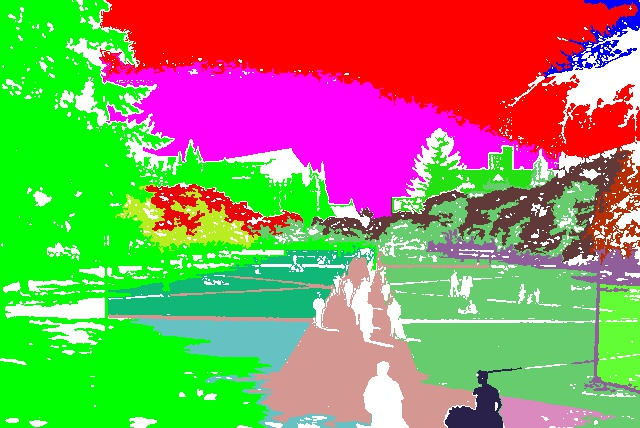
\includegraphics[scale=0.3]{report/p4-3-1-X10}}
		}
		\label{fig:bfs10}
	}
	\quad
	\subfloat[X = 20.]{
		{
			\setlength{\fboxsep}{1pt}
			\setlength{\fboxrule}{1pt}
			\fbox{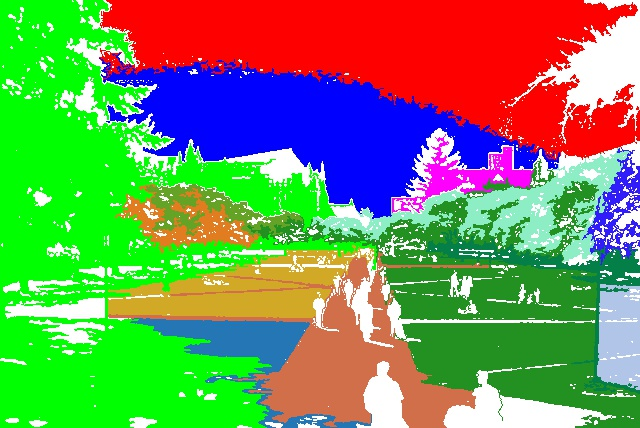
\includegraphics[scale=0.3]{report/p4-3-1-X20}}
		}
		\label{fig:bfs20}
	}
	\caption{Connected regions extracted using the BFS explorer for different $X$ values.}
	\label{fig:bfs}
\end{figure}

	In Figure \ref{fig:bfs} each colour represents a connected region and Figure \ref{fig:bbox} shows their bounding boxes. Regions that are too small don't really describe enough of a feature to be relevant, and thus are discarded, in Figure \ref{fig:bfs} the white colour is used to represent the discarded ones.

\newpage

\begin{figure}[!h]
	\centering
	\subfloat[X = 0.]{
		{
			\setlength{\fboxsep}{1pt}
			\setlength{\fboxrule}{1pt}
			\fbox{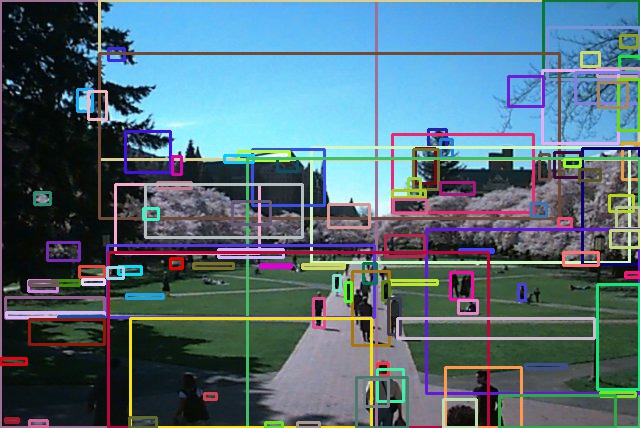
\includegraphics[scale=0.3]{report/p4-3-2-B00}}
		}
		\label{fig:bbox00}
	}
	\quad
	\subfloat[X = 6.]{
		{
			\setlength{\fboxsep}{1pt}
			\setlength{\fboxrule}{1pt}
			\fbox{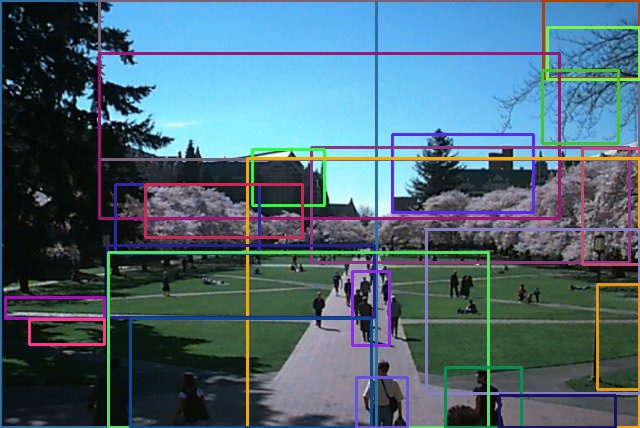
\includegraphics[scale=0.3]{report/p4-3-2-B06}}
		}
		\label{fig:bbox06}
	}
	\quad
	\subfloat[X = 10.]{
		{
			\setlength{\fboxsep}{1pt}
			\setlength{\fboxrule}{1pt}
			\fbox{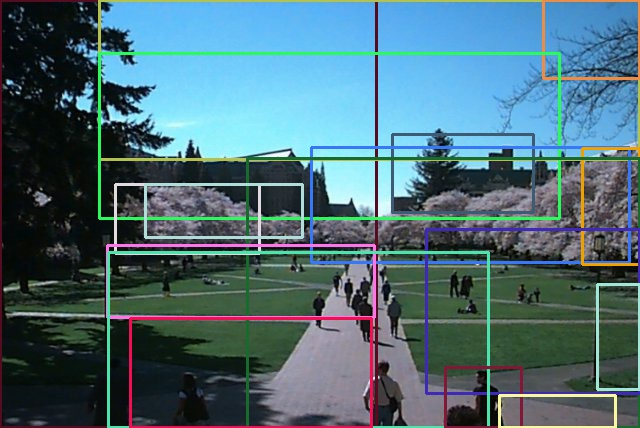
\includegraphics[scale=0.3]{report/p4-3-2-B10}}
		}
		\label{fig:bbox10}
	}
	\quad
	\subfloat[X = 20.]{
		{
			\setlength{\fboxsep}{1pt}
			\setlength{\fboxrule}{1pt}
			\fbox{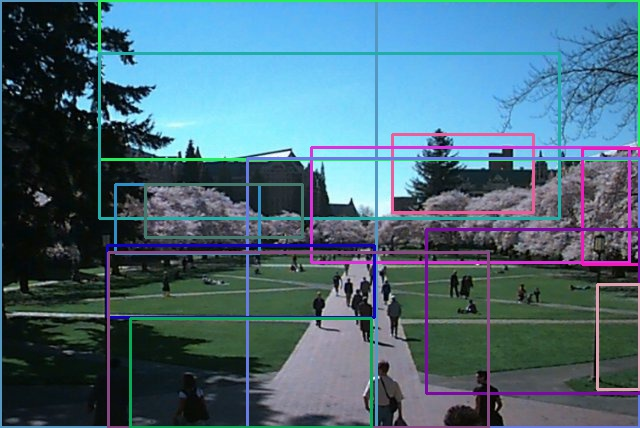
\includegraphics[scale=0.3]{report/p4-3-2-B20}}
		}
		\label{fig:bbox20}
	}
	\caption{Bouding box of each region calculated with different $X$ values.}
	\label{fig:bbox}
\end{figure}

	A region is considered too small if its size is smaller than the multiplication of a factor $X$ by the average region size, this value was chosen based on our analysis of the yielded results given by the input data set.
	
	In Figure \ref{fig:bfs00} and Figure \ref{fig:bbox00} the value of $X$ is set to zero and it is possible to observe regions as big as one pixel line being taken, which is counter productive towards our goal as they don't describe something relevant. In Figure \ref{fig:bfs06} and Figure \ref{fig:bbox06}, with $X = 6$, smalls non-discriminative regions are still being selected, like the tree on the right upper side of the image, the human carrying a bag in the bottom centre (Figure \ref{fig:bfs06} shows that only the bag and pants were selected) and a few smalls patches of grass in the left bottom side, all of those describes non-discriminative features that could diminish the final result. In Figure \ref{fig:bfs10} and Figure \ref{fig:bbox10}, where $X = 10$, there are still some non-discriminative regions being selected, like half of the tree in the right upper corner, but they are few and contrasted with a majority of somewhat big, discriminative regions, like the cherry trees, the buildings in the back and the path in the centre. In Figure \ref{fig:bfs20} and Figure \ref{fig:bbox20}, with $X = 20$, almost all the small ignorable regions were discarded and it performed well in this image, but since it was a too big value it could start eliminating discriminative regions on other images, diminishing their accuracy, this and the inefficiency of the small values to determine good sized regions was the reason why we chose $X = 10$.

\newpage

	These regions will be used as descriptors of the image, and compared later on, to do so it is necessary to describe each region, in a data structure,  a vector and the following information were selected to do so: region size \textbf{(size)}, region mean color \textbf{(mean\_color)}, region centroid \textbf{(centroid)}, region bounding box \textbf{(bounding\_box)} and some texture features for the region patch. The patch of the texture features were extracted using the delimitations of their bounding boxes and are composed of: contrast \textbf{(contrast)}, correlation \textbf{(correlation)}, dissimilarity \textbf{(dissimilarity)}, energy \textbf{(energy)} and entropy \textbf{(entropy)}. These components were extracted using the co-occurrence matrix, applied to the region patch, and they tend to describe correlation between pixels in the region, Figure \ref{fig:cent} illustrate the centroid position of each region. The bold names will be explained in the next section.

\begin{figure}[!h]
	\centering
	\subfloat[X = 0.]{
		{
			\setlength{\fboxsep}{1pt}
			\setlength{\fboxrule}{1pt}
			\fbox{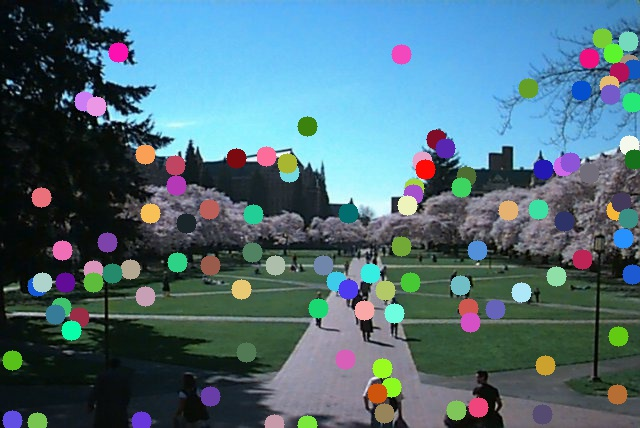
\includegraphics[scale=0.3]{report/p4-3-3-C00}}
		}
		\label{fig:cent00}
	}
	\quad
	\subfloat[X = 6.]{
		{
			\setlength{\fboxsep}{1pt}
			\setlength{\fboxrule}{1pt}
			\fbox{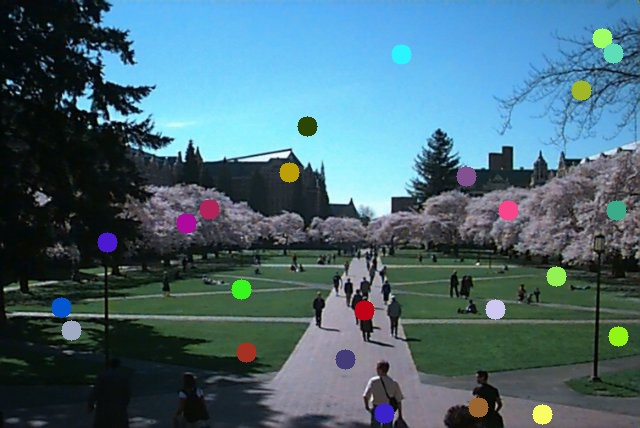
\includegraphics[scale=0.3]{report/p4-3-3-C06}}
		}
		\label{fig:cent06}
	}
	\quad
	\subfloat[X = 10.]{
		{
			\setlength{\fboxsep}{1pt}
			\setlength{\fboxrule}{1pt}
			\fbox{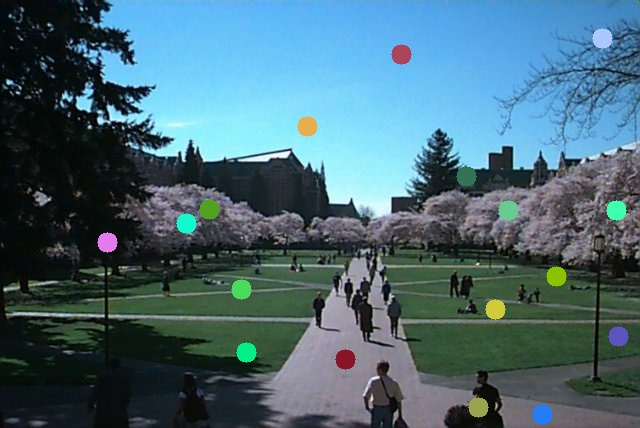
\includegraphics[scale=0.3]{report/p4-3-3-C10}}
		}
		\label{fig:cent10}
	}
	\quad
	\subfloat[X = 20.]{
		{
			\setlength{\fboxsep}{1pt}
			\setlength{\fboxrule}{1pt}
			\fbox{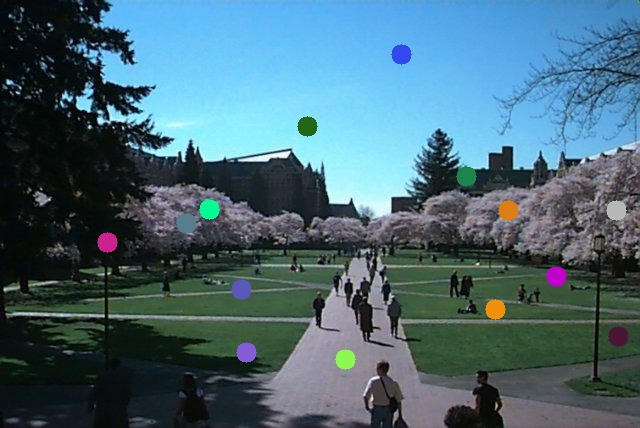
\includegraphics[scale=0.3]{report/p4-3-3-C20}}
		}
		\label{fig:cent20}
	}
	\caption{Centroid of each image calculated with different $X$ values.}
	\label{fig:cent}
\end{figure}

% =========================================================================================================================================================

\newpage

\textbf{\LARGE Question 3 - Distance Measure} \\

In order to create a content-based image retrieval, we developed a distance measurement for our collected descriptors that are based on the regions obtained by the connected components algorithm. The distance formula used was a simple difference method over the features size, mean color, and the textures features for each region. Moreover, euclidean distance was used for compute the centroids distance. \\

Every region is described by a single value that is composed by the average between all the differences found in the features descriptors for that region. Two different average process are taken, the first one is between the feature vector for the textures obtained by the co-occurrence matrix.And, the other one is an average operation between all the features for that region. \\

As images might contain different number of regions, a region is compared to all others and the minimum distance is chosen to represent the region. After determining all the distances for the regions, a average is performed between them giving a single value to classify the similarity between both images. Smaller values mean more correlation, while higher values describe more distinctive images. The Figure \ref{fig:simpleAvr} shows a result for some queried images. 

\begin{figure}[!h]
	\centering
	\subfloat[]{
		{
			\setlength{\fboxsep}{1pt}
			\setlength{\fboxrule}{1pt}
			\fbox{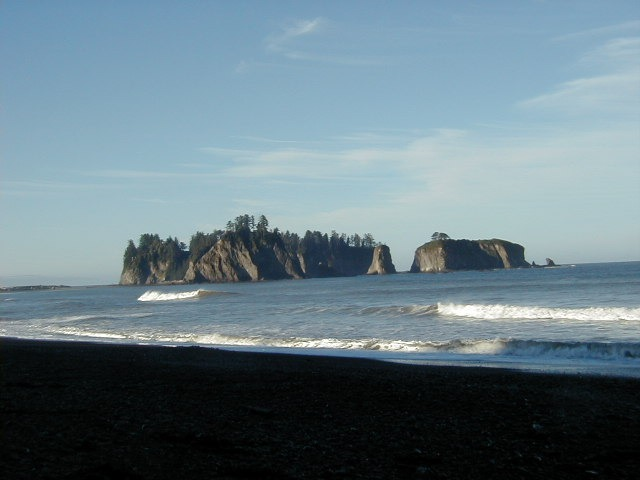
\includegraphics[scale=0.3]{report/beach_2.jpg}}
		}
	}
	\subfloat[]{
		{
			\setlength{\fboxsep}{1pt}
			\setlength{\fboxrule}{1pt}
			\fbox{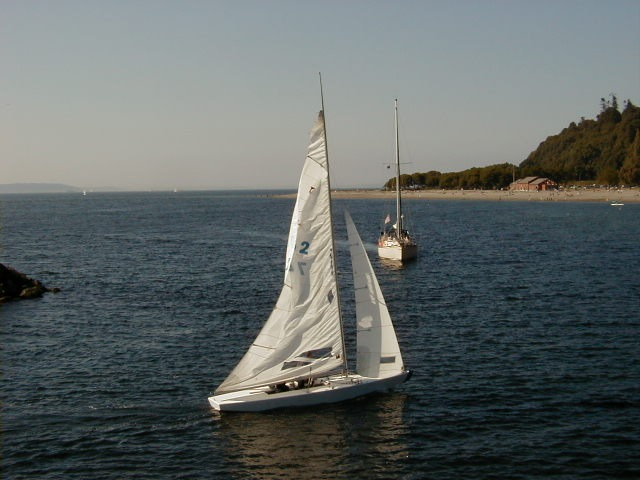
\includegraphics[scale=0.3]{report/boat_2.jpg}}
		}
	}
	\subfloat[]{
		{
			\setlength{\fboxsep}{1pt}
			\setlength{\fboxrule}{1pt}
			\fbox{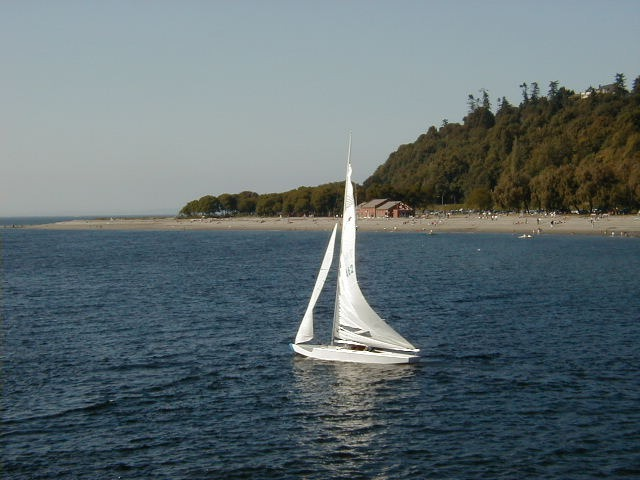
\includegraphics[scale=0.3]{report/boat_5.jpg}}
		}
	}
	\subfloat[]{
		{
			\setlength{\fboxsep}{1pt}
			\setlength{\fboxrule}{1pt}
			\fbox{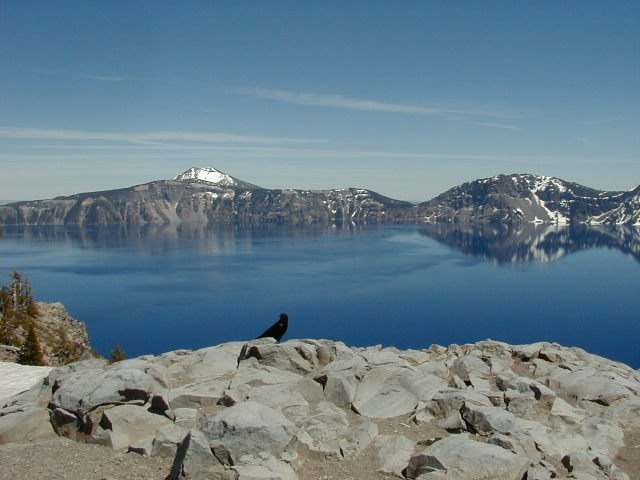
\includegraphics[scale=0.3]{report/crater_1.jpg}}
		}
	}
	\caption{Difference between keypoint detection methods.}
	\label{fig:simpleAvr}
\end{figure}

\end{document}
